\section{Durchführung}
\label{sec:Durchführung}

\subsection{Aufgabenstellung}
Bestimmung

   \begin{enumerate}
     \item der Zeitabhängigkeit der Amplitude eines gedämpften Schwingkreises
     und seines effektiven Dämpfungswiderstandes
     \item von $R_{ap}$ für den aperiodischen Grenzfall
     \item der Frequenzabhängigkeit von $U_C$
     \item der Frequenzabhängigkeit der Phase \varphi zwischen Erregerspannung
     und $U_C$
     \item der Frequenzabhängigkeit der Impedanz
   \end{enumerate}


\subsection{Gerätedaten}
Für alle Messungen wurde Gerät 2 verwendet mit folgenden Spezifikationen:\\
$L= (10,11\pm 0.03)\symup{mH}$, $C=(2,098 \pm 0.006)\symup{nF}$,
$R_1 =(48,1 \pm 0,1) \symup{\Omega}$, $R_2=(509,5 \pm 0,5)\symup{\Omega}$

\subsection{Messung der Kondensatorspannung in Abhängigkeit von der Zeit}
Zunächst wird der Schwingkreis mittels eines Nadelimpuls kurz angeregt,

da kein Nadelimpulsgenerator zur Verfügung stand, wurde dieser mit einer
Rechteckspannung mit klein möglichster Impulsbreite moduliert.

Dies dient dazu dem System eine Anfangsenergie zu übergeben. Die Frequenz des
Generators wird mit ca. 600 Hz so gering gewählt, dass die Schwingung vor einer
erneuten Anregung nahezu vollständig abgeklungen ist. Die am Kondensator
anliegende Spannung $U_C$ wird hierbei mit Hilfe eines digitalen Oszilloskops
aufgezeichnet.

\begin{figure}
  \centering
  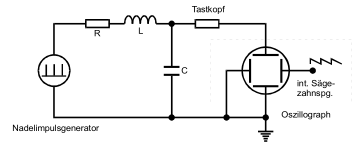
\includegraphics[height= 4cm]{./logos/Amplitude_Schaltung.PNG}
  \caption{Zur Erfassung der Schwingung des angeregten RCL-Kreises verwendete
  Schaltung mit $R = R_1$ aus Quelle \cite{sample}}
  \label{fig:5a}
\end{figure}

\subsection{Grobe Messung des Dämpfungswiderstandes}
Da im folgenden $R_{ap}$ bestimmt werden soll, wird $R$ in Abb.\ref{fig:5a} als
frei zwischen $0\symup{\Omega}$ und $10\symup{k\Omega}$ einstellbar realisiert.
$R_{ap}$ lässt
sich näherungsweise bestimmen, indem zuerst $R = 10\symup{k\Omega}$ gewählt wird. Nun
wird der Widerstand reduziert, bis eine schwache Schwingung
erkennbar ist, um ihn dann wieder zu erhöhen, bis die Schwingung
gerade eben verschwindet. An diesem Punkt hat man $R_{ap}$ in grober Näherung
gemessen.

\subsection{Messung der Frequenzabhängigkeit der Kondensatorspannung}
Zur Messung der Frequenzabhängigkeit der am Kondensator auftretenden Spannung
stellt man den Impulsgenerator aus Abb.\ref{fig:5a} so um, dass er eine
Sinusspannung generiert. Desweiteren wird $R=R_2$ gewählt. Nun wird die
Kondensatorspannung bei unterschiedlichen Frequenzen protokolliert, wobei
zusätzlich das Ausgangssignal $U$ des Generators direkt gemessen wird, um eine
eventuell im Tastkopf entstehende Phasenverschiebung herausrechnen zu können.
Ebenfalls berücksichtigt werden muss der Eigenwiderstand der verwendeten Geräte.

\subsection{Messung der Frequenzabhängigkeit der Phase zwischen Erreger-und Kondensatorspannung}
Erneut werden Kondensator- und Eingangsspannung für unterschiedliche Frequenzen
aufgenommen. Diesmal jedoch werden sie am Oszilloskop auf ihren Gangunterschied
untersucht mittels des Cursors, welcher sich auf die Extremstellen der Signale
setzen lässt und den Zeitunterschied zwischen beiden liefert. Wieder gilt $R=R_2$.
In dieser Messreihe wurden 12 Werte im Frequenzbereich von ca. 101 kHz bis 0,2 kHz
gemessen.


\subsection{Messung der Frequenzabhängigkeit des Scheinwiederstandes}
Zuletzt wird die Impedanz des Aufbaus ermittelt, indem am Oszilloskop die vom
Generator ausgegebene Spannung und der Stromfluss im RCL-Kreis in Abhängigkeit
von der Frequenz der Anregung aufgenommen werden.
